\documentclass[12pt]{article}
\usepackage[utf8]{inputenc}
\usepackage[english]{babel}
\usepackage[dotinlabels]{titletoc}
\usepackage[nottoc]{tocbibind}
\usepackage{mathptmx}
\usepackage{amsmath, amssymb}
\usepackage{geometry, titlesec, setspace}
\usepackage{graphicx, caption, subcaption}
\usepackage{hyperref, natbib}
% Journals
\newcommand{\aap}{A\&A}
\newcommand{\aj}{AJ}
\newcommand{\apj}{ApJ}
\newcommand{\araa}{ARA\&A}
\newcommand{\mnras}{MNRAS}
\newcommand{\nat}{Nature}
\newcommand{\pasa}{PASA}
\newcommand{\pasp}{PASP}
\newcommand{\physrep}{PhR}
\newcommand{\prd}{PhRvD}
\newcommand{\rpph}{RPPh}

% Page formatting
\geometry{
	left=1.25in,
	right=1.25in,
	top=1in,
	bottom=1in}
\hypersetup{
	colorlinks=true,
	citecolor=blue,
	filecolor=blue,
	linkcolor=blue,
	urlcolor=blue
}
\setlength{\footnotesep}{10pt}
\setlist{noitemsep}

% Fixing titlesec and hyperref interaction
\makeatletter
\def\ttl@useclass#1#2{%
\@ifstar
{\ttl@labeltrue\@dblarg{#1{#2}}}
{\ttl@labeltrue\@dblarg{#1{#2}}}}
\makeatother

% Image setup
\graphicspath{{figs/}}
\captionsetup[figure]{labelfont={bf}, font={small, stretch=1.3}, name={Figure}, labelsep=period}

% Section and subsection headings
\titleformat{\section}{\normalsize\bfseries\centering}{}{0em}{}
\titleformat{\subsection}{\normalsize\itshape\centering}{}{0.75em}{}
\newcommand{\nocontentsline}[3]{}
\newcommand{\tocless}[2]{\bgroup\let\addcontentsline=\nocontentsline#1{#2}\egroup}
\renewcommand{\contentsname}{Table of Contents}
\renewcommand{\abstractname}{{\normalsize\bfseries\centering{Abstract}}}
\renewcommand{\bibsection}{}

% For figures
\makeatletter
\setlength{\@fptop}{0pt plus 1fil}
\setlength{\@fpbot}{0pt plus 1fil}
\makeatother

% For formatting text and math
\let\vec\mathbf
\newcommand{\code}[1]{{\fontfamily{qcr}\selectfont#1}}
\newcommand{\red}[1]{\textcolor{red}{#1}}
\newcommand{\note}[1]{\textcolor{violet}{#1}}

% Special commands
\newcommand{\HI}{H\,\textsc{i}}
\newcommand{\OI}{O\,\textsc{i}}
\newcommand{\heraqm}{\code{hera\textunderscore qm}}
\newcommand{\herapspec}{\code{hera\textunderscore pspec}}
\newcommand{\herasim}{\code{hera\textunderscore sim}}
\newcommand{\pyuvdata}{\code{pyuvdata}}

\begin{document}
\doublespacing
\begin{center}
Environmental Systematics and the Impact on \\ 21-cm Epoch of Reionization Measurements \\
by \\
Lily Whitler \\
has been approved \\
Spring 2019 \\[0.1\textheight]

\begingroup
\renewcommand{\arraystretch}{0.7}
\begin{tabular}{p{1cm}p{3.5in}p{1cm}}
	& \centering APPROVED: & \\
	& & \\ & & \\
	& \hrulefill & \\
	& \hfill Daniel Jacobs, Director & \\
	& & \\ & & \\
	& \hrulefill & \\
	& \hfill Judd Bowman & \\
	& & \\ & & \\
	& \hrulefill & \\
	& \hfill Adam Beardsley &
\end{tabular} \\[0.075\textheight]
\begin{tabular}{p{1cm}p{3.5in}p{1cm}}
	& \centering ACCEPTED: & \\
	& & \\ & & \\
	& \hrulefill & \\
	& \hfill Dean, Barrett, The Honors College &
\end{tabular}
\endgroup
\end{center}
\thispagestyle{empty}
\newpage
\pagenumbering{arabic}

\begin{center}
	{\Large Environmental Systematics and the Impact on \\ 21-cm Epoch of Reionization Measurements} \\
	by \\
	Lily Whitler \\[0.15\textheight]
	
	A Thesis Presented in Partial Fulfillment \\
	of the Requirements for Graduation from \\
	Barrett, the Honors College \\[0.15\textheight]
	
	Committee: \\
	Daniel Jacobs, Director \\
	Judd Bowman \\
	Adam Beardsley \\[0.2\textheight]
	
	ARIZONA STATE UNIVERSITY \\
	April 2019
\end{center}
\thispagestyle{empty}

\clearpage
\pagenumbering{roman}

\begingroup
\hypersetup{
	colorlinks=true,
	citecolor=DarkBlue,
	filecolor=black,
	linkcolor=black,
	urlcolor=DarkBlue
}
\tableofcontents
\listoffigures
\listoftables
\endgroup
\newpage

\begin{abstract}
\end{abstract}

\clearpage
\pagenumbering{arabic}

\section{Introduction} \label{sec:intro}

\subsection{A Brief History of the Universe} \label{subsec:universe}

Immediately after the Big Bang, the universe was a hot plasma of fundamental particles. Now, nearly 14 billion years later, it is populated with a rich variety of \red{objects}, from massive galaxy clusters all the way down to our own solar system and its planets. However, the \red{evolutionary} path the universe took from the Big Bang to now is not entirely clear.

In the early universe, matter was hot and ionized. Photons scattered off of free particles, rendering the universe opaque to electromagnetic radiation. This lasted until approximately 380,000 years after the Big Bang, when the universe had expanded and cooled sufficiently for electrons to become bound to atomic nuclei during recombination. When recombination was complete, photons were able to propagate freely through space, subject only to cosmological redshift. Today, we see photons from this era as the cosmic microwave background (CMB).

Immediately following the release of the CMB and lasting until several hundred million years after the Big Bang was the cosmic Dark Ages. During this era, though photons were free to propagate, no stars, galaxies, or other sources of radiation had yet formed. The only sources of information we have from the Dark Ages are CMB photons and emission from neutral hydrogen.

The transition between the Dark Ages and the subsequent Epoch of Reionization (EoR) was marked by the \red{emergence} of the first luminous sources. During the EoR, ultraviolet (UV) radiation from these objects ionized the intergalactic medium (IGM) around them. The EoR ended when the IGM was fully ionized, thus completing the final major phase change of hydrogen in the universe.

Figure \ref{fig:timeline} shows an illustration of this evolution. The \textit{Planck} satellite and its predecessors, the \red{Cosmic Background Explorer [italics?]} and \textit{Wilkinson Microwave Anisotropy Probe}, have measured the temperature anisotropies in the CMB, providing a wealth of information about the universe just a few hundred thousand years after its \red{birth}. On the other end of cosmic history, the Hubble Deep Fields have probed some of the oldest known galaxies. \red{However, most of the Dark Ages and EoR still lack observational constraints.}

\begin{figure}[tb]
	\centering
	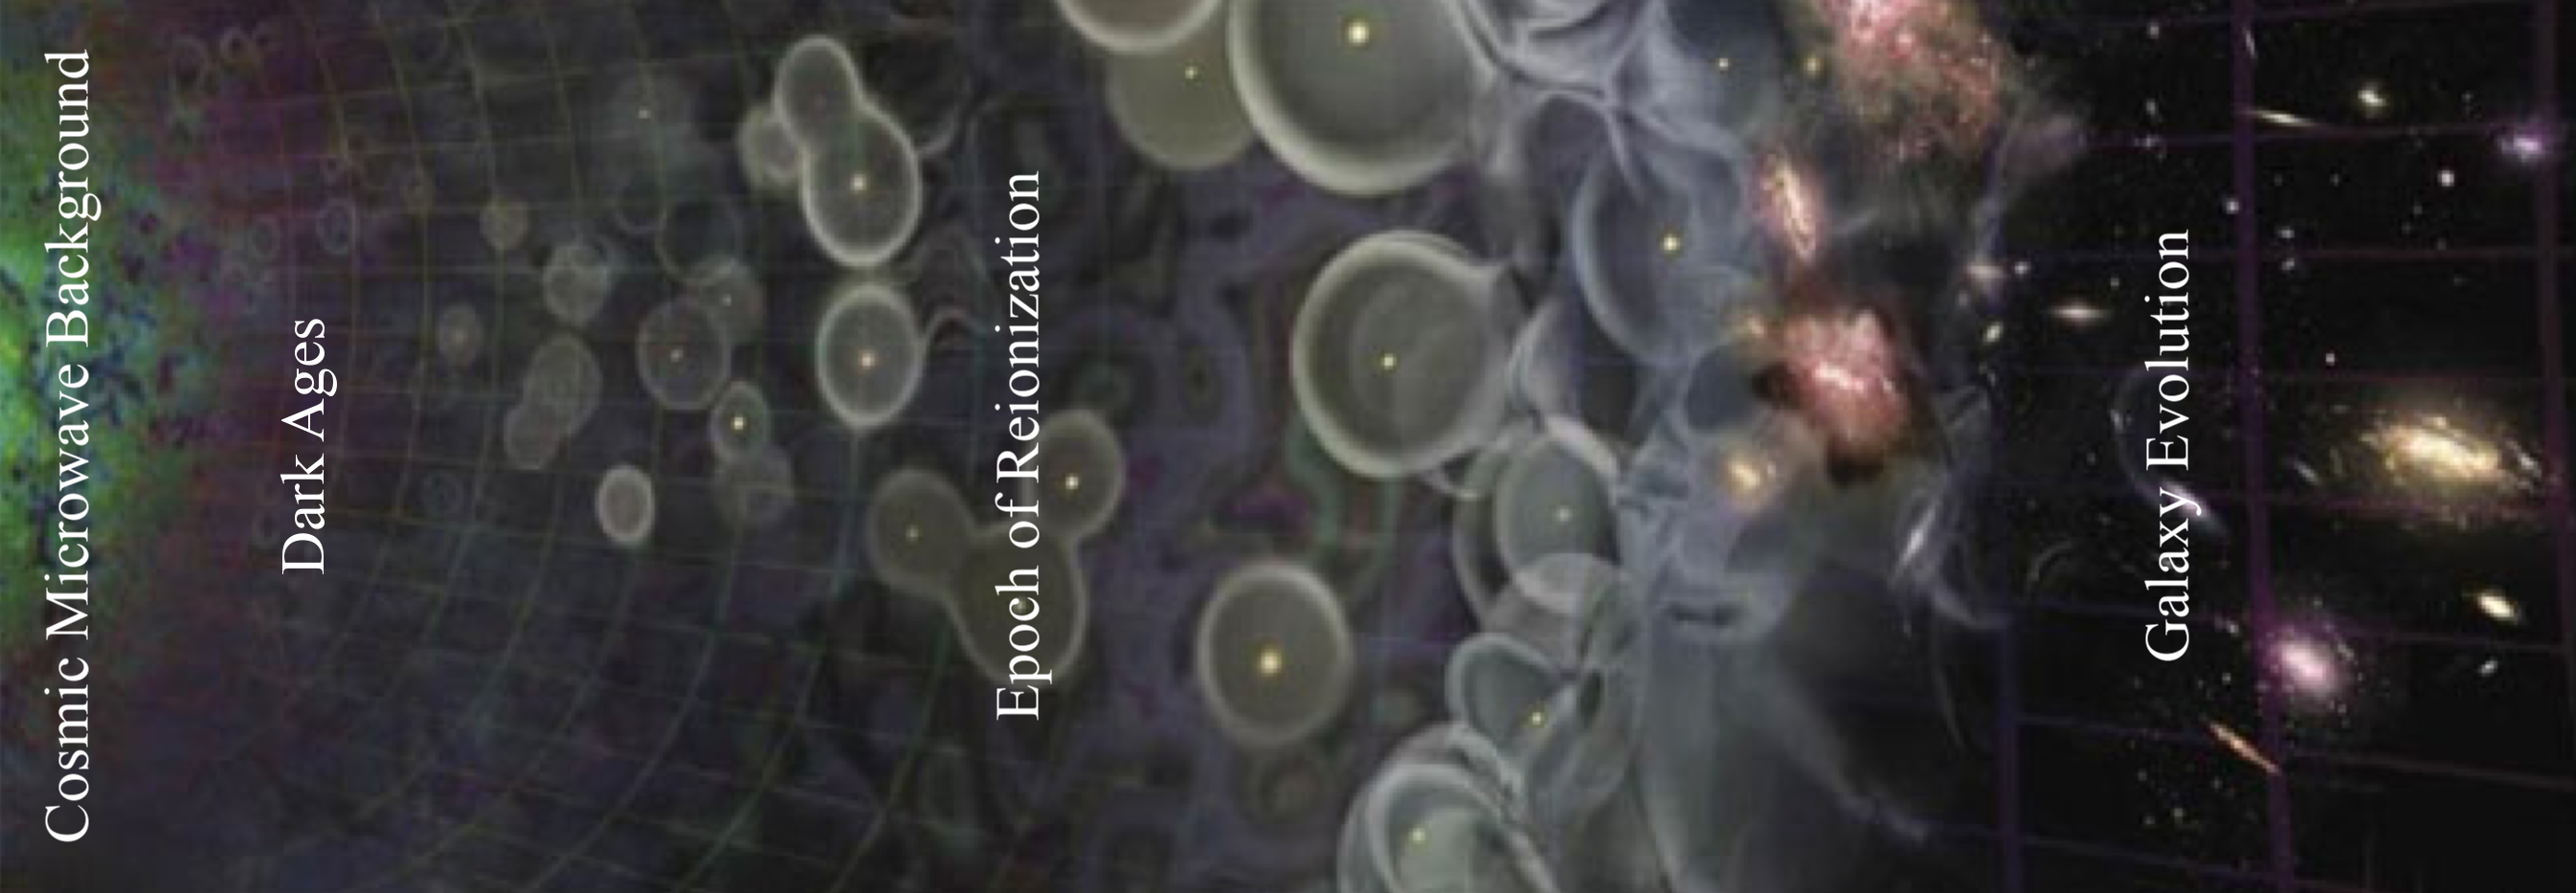
\includegraphics[width=\textwidth]{timeline.png}
	\caption[History of the universe]{A visualization of cosmic evolution. Image originally from \cite{loeb2006}.}
	\label{fig:timeline}
\end{figure}

\subsection{The Epoch of Reionization} \label{subsec:eor}

The EoR is the period in cosmic history during which the intergalactic medium, which had been neutral since recombination, was ionized by the very first luminous sources. This era, along with the Dark Ages, is the bridge between \red{our knowledge of} the CMB and the universe today.

Though the EoR is largely observationally \red{unconstrained}, theoretical studies have constructed a broad \red{account} of the ionization process. UV photons from the earliest stars, galaxies, or quasars ionized the gas in their immediate neighborhood, and as individual objects continue ionizing their surroundings, these bubbles of ionized gas grew in size and eventually began to overlap. As the EoR progressed, the bubbles continued to grow and overlap until the IGM was fully ionized.

This \red{qualitative} picture is generally accepted, but answering more detailed questions such as ``What is the timeline of reionization?'', ``What was the topology? Were there a lot of small bubbles or did a few large ones dominate?'', or even ``What exactly were the ionizing sources?'' \red{[this can most definitely be worded better]} will require observations of this era.

\subsection{Observational Constraints on the Epoch of Reionization} \label{subsec:probes}

\cite{fan2006} constrained the end of reionization to be around $z \sim 6$, primarily via observations of high-redshift quasars. This approach will continue to place tighter \red{limits} on the \red{tail end} of reionization, especially since deep surveys with the upcoming \textit{James Webb Space Telescope} and other ground- and space-based instruments will enable detections of statistically significant samples of these high-redshift objects. However, the \red{[something] luminosity function limits the detection of quasars above $z \gtrsim 7$, thus limiting our ability to probe the earlier part of the EoR with these objects \textit{(citation)}}.

Other probes of the EoR include gamma ray bursts and metal absorption line systems. High-redshift gamma ray bursts exhibit troughs \red{blueward} of Lyman alpha (Ly$\alpha$) in their spectra due to absorption by intervening neutral hydrogen, thus serving as a probe of the ionization state of the IGM \citep[e.g.,][]{gallerani2008}. Early star formation enriches the interstellar medium and the IGM with heavy elements, which can be used either to probe the properties of the stellar populations that ionized the universe or to directly trace the ionization history. For example, \cite{oh2002} \red{proposed} the use of the \OI~line at 1302 \AA, since \OI~and H have almost identical ionization potentials and \OI~is expected to be in tight charge exchange equilibrium with H.

Both the large-scale polarization of the CMB and the small-scale kinetic Sunyaev-Zel'dovich (kSZ) effect place some constraints on the onset and topography of reionization \citep{fan2006}. CMB photons undergo Thomson scattering off of free electrons produced by the ionization of hydrogen which causes the emission to polarize. This interaction can be quantified by the optical depth of reionization, and thus the redshift. Primary CMB anisotropies are suppressed by this polarization, so measuring the polarization caused by CMB photons Thomson scattering during reionization constrains the onset of the EoR \citep[e.g.,][]{zaldarriaga1997, roy2018}. The kSZ effect, on the other hand, is due to inverse Compton scattering of ionized electrons in the IGM and introduces secondary temperature anisotropies on small angular scales, which is a tracer of the \red{patchiness} of reionization \citep{fan2006, park2013, roy2018}.

As useful as the CMB is as a probe of the EoR, it is essentially a two-dimensional snapshot of the universe taken at one time in cosmic history. Although the CMB has imprints of other eras, specifically the EoR, on it, a three-dimensional map would contain much information. \red{I need more stuff here, but moving on to the 21-cm stuff for now...}

\subsection{21-cm Cosmology} \label{subsec:21cm}

Neutral hydrogen emits a photon with a wavelength of 21 centimeters during its so-called ``spin-flip transition.'' In the ground state of neutral hydrogen, an electron is bound to a proton, each of which has an intrinsic quantum spin due to their magnetic dipole moments. The spin of the electron can be either parallel or antiparallel to the proton's spin, and the parallel state is slightly higher in energy. The transition from the parallel to the antiparallel state is called the spin-flip transition and results in the emission of a 21-cm photon. \red{The energy difference between these two states is $\sim 5.87$ $\mu$eV, a tiny fraction of the 13.6 eV necessary to ionize hydrogen once, making the 21-cm line one of the only ways to probe the very low-energy environment of the Dark Ages and early stages of the EoR.}

Due to the expansion of the universe, the observed wavelength of the 21-cm line is redshifted to longer wavelengths, which can be traced back to a specific time in cosmic history. This redshift evolution provides a full three-dimensional probe of the EoR. Theoretical studies of the EoR place the EoR approximately between $z \sim 20 - 6$ \red{(This may not be quite right. Also, citations??)}, which corresponds to observed wavelengths of approximately 1.5 -- 4.5 meters. The spin flip transition has a very small transition rate of $2.9 \times 10^{-15}$ s$^{-1}$, or about one transition every 10 million years, but fortunately, hydrogen is incredibly ubiquitous in the universe so we can still use this line as an EoR probe.

Actually measuring 21-cm emission from the EoR, however, is an exercise in extreme precision. Synchrotron emission from our own galaxy and other extragalactic sources dominates the frequency band of interest, creating foregrounds that are several orders of magnitude brighter than the 21-cm signal is expected to be. These foregrounds are the primary challenge that all 21-cm experiments must overcome to detect the EoR. However, the environment and the instrument can introduce other \red{systematics}, such as radio frequency interference (RFI), ionospheric effects, and cable reflections, that further complicate the measurement.

\subsection{Radio Frequency Interference} \label{subsec:rfi}

Interference from sources including FM radio, satellite and aircraft communications, television transmissions, and even nearby weather events (e.g., lightning) is exceptionally bright and can easily contaminate the results of any cosmological measurement. \red{Unfortunately}, since it is typically man-made, it is also everywhere that humans are.

There are a few ways to mitigate RFI. First, instruments can be built in remote areas to minimize contact with human-made interference. Then, RFI can be removed after taking observations with software that detects and masks out (``flags'') data it identifies as being contaminated. Steps further along in the data reduction and analysis process ignore this flagged data.

There are currently several radio interferometers making observations towards a 21-cm power spectral EoR detection, some of which are located in remote places of the world and all \red{(I think)} of which use some sort of RFI excision software. The Hydrogen Epoch of Reionization Array (HERA), located in the Karoo Desert in South Africa, does both.

\subsection{The Hydrogen Epoch of Reionization Array} \label{subsec:hera}

\begin{figure}[tb]
	\centering
	\begin{subfigure}{0.48\textwidth}
		\centering
		{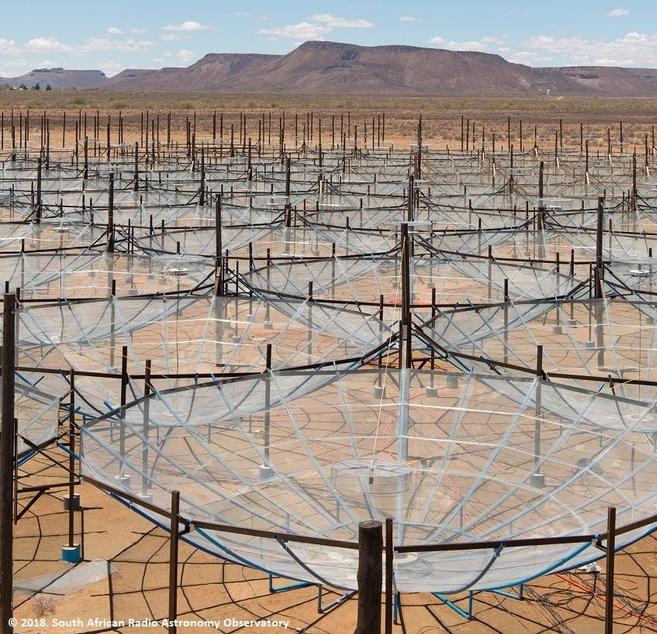
\includegraphics[width=\textwidth]{hera.png}}
	\end{subfigure} \hfill
	\begin{subfigure}{0.48\textwidth}
		\centering
		{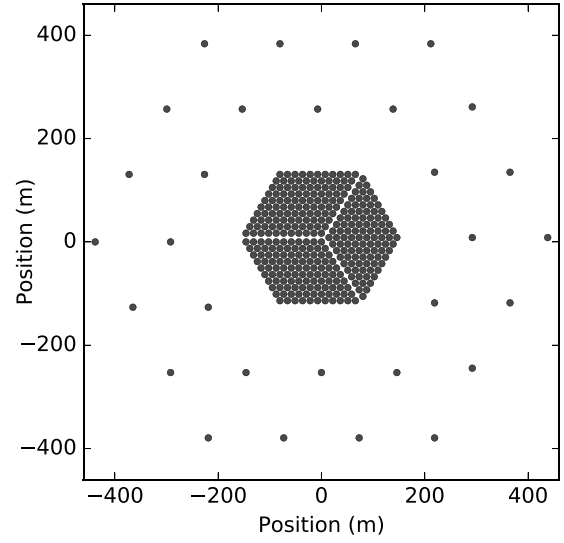
\includegraphics[width=\textwidth]{hera_map.png}}
	\end{subfigure}
	\caption[The Hydrogen Epoch of Reionization Array]{Left: A photo of HERA as of late 2017 -- early 2018. HERA will observe the periods prior to and during the EoR via the redshifted 21-cm line from the IGM. Image courtesy of the South African Radio Astronomy Observatory. Right: A map of the completed array, composed of 320 central elements and 30 outriggers \citep{deboer2017}.}
	\label{fig:hera}
\end{figure}

HERA (left panel of Figure \ref{fig:hera}) is one of several radio interferometers designed to study the large-scale structure during the EoR via measurements of the redshifted 21-cm line \citep{deboer2017}---others include the Low Frequency Array \citep[LOFAR;][]{vanHaarlem2013} and the Murchison Widefield Array \citep[MWA;][]{tingay2013}. HERA builds upon preceding instruments, such as the MWA and the Donald C. Backer Precision Array for Probing the Epoch of Reionization \citep[PAPER;][]{parsons2010}, and will pave the way for future experiments such as the Square Kilometer Array \cite[SKA; e.g.,][]{mellema2013}.

When complete, HERA will be \red{composed} of 350 14-meter dishes with a dense 320-element hexagonal core and 30 outriggers (right panel of Figure \ref{fig:hera}). The dense \red{configuration} was chosen to maximize sensitivity to the diffuseness of the 21-cm signal, which will be sampled primarily by short baselines. \red{The redundancy of the hexagonal shape increases sensitivity and the efficacy of the delay spectrum approach for separating and rejecting foreground-contaminated modes \textit{(this is apparently a PAPER thing??---citation?)} and allows for the redundant calibration technique developed and pioneered in \cite{liu2010} and \cite{zheng2014}. [explain this entire thing more (or cut it)]}

\section{Methods} \label{sec:methods}

\subsection{RFI Excision Strategies} \label{subsec:rfi_excision}

\begin{figure}[tb]
	\centering
	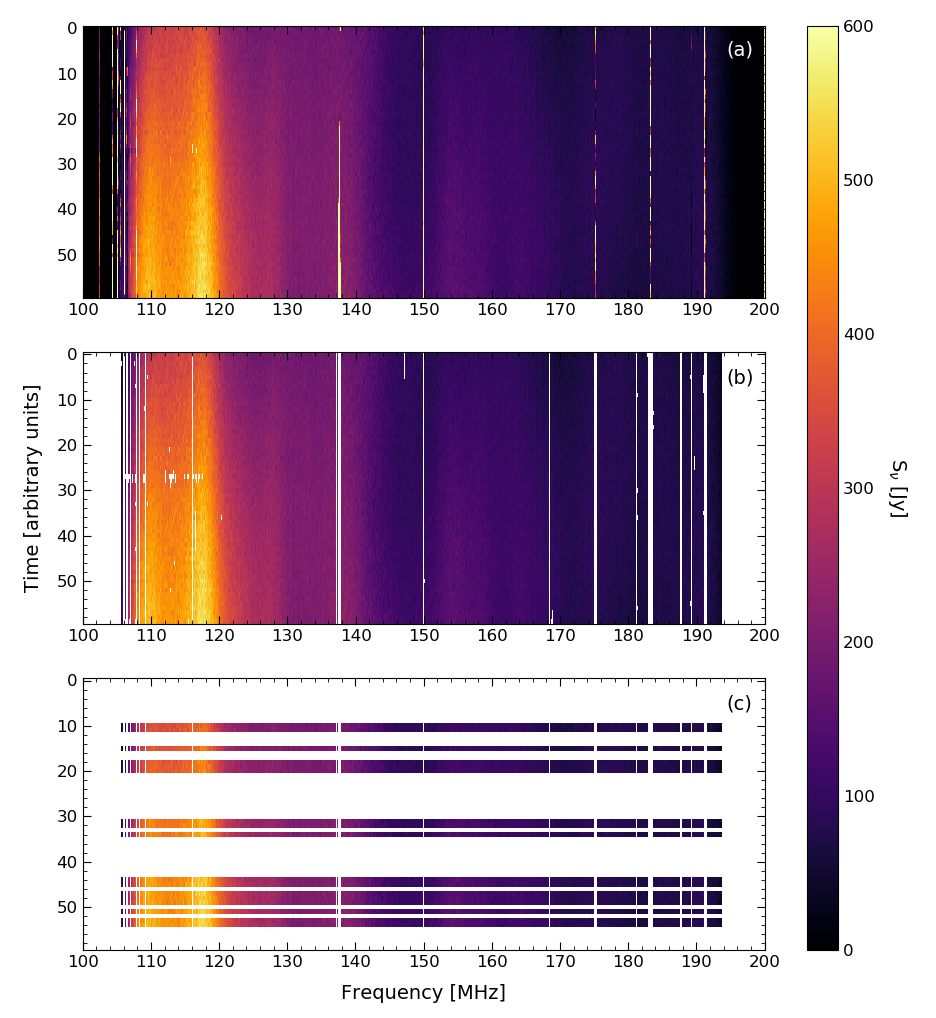
\includegraphics[width=\textwidth]{flagging_steps.png}
	\caption[Steps for flagging RFI]{\red{Something about how we go about flagging RFI before calculating the power spectrum}}
	\label{fig:rfi_flagging}
\end{figure}

\red{Initial flagging with XRFI}

\red{Flag broadcasting with \code{hera\textunderscore pspec}}

\subsection{Calculating the Power Spectrum} \label{subsec:calc_ps}

\subsection{Modelling HERA Data} \label{subsec:modelling}

\red{Making \code{hera\textunderscore sim} talk to \code{pyuvdata}}

\section{Results}

\section{Conclusions}

\bibliographystyle{aasjournal}
\bibliography{refs}
\end{document}